\documentclass[11pt]{extarticle}

\usepackage[hypertexnames=false]{hyperref}
\usepackage{tikz}

\hypersetup{
    colorlinks,
    citecolor=black,
    filecolor=black,
    linkcolor=black,
    urlcolor=black,
    linktoc=all
}

\renewcommand{\thesection}{\Alph{section}}
\renewcommand{\theHsection}{\Alph{section}}

\title{\Huge{Documentation for the dungeon project}}
\author{Quentin GUEZ}
\date{}

\begin{document}

\maketitle

\tableofcontents

\clearpage

\part{Game description}

\section{Explanation of the game}

You are controlling Thorn, a young adventurer and you have a new quest in this adventure. You's trying to gather all the four Statues of Youth. Those would let you make any wish he wants. Unfortunately, those statues are being kept by the terrible Girk. He's been keeping them for years as his glorious treasure. Now has come the time for you to pick them up and make any wish come true.

On your way to the statues, you will face many dangers. You'll start in a outside where there's only one door facing you. You will therefore have to make choices about where you choose to go. 

If you meet an enemy, you will have a choice : whether trying to flee but with a low chance of success, or you can directly attack and bravely face the danger. But be careful, you don't know how the strong the enemy is yet. 

If you get lucky on your way, you might find a magic key that can unlock any door. But be aware that you can only use one per door. You can also find weapons or potions on your way so watch your steps.

\section{List of the functionnalities}

\begin{itemize}
    \item move between rooms
    \item play music
    \item describe each room's name
    \item check the player's stats
    \item fight an enemy 
    \item choose an attack
    \item double attack with random chance of success
    \item possibility to flee and escape the enemy as long as you don't go back to the room
    \item a music and a description for each transition
    \item rooms can be locked or opened
    \item possibility to find items (key, potion, statue)
    \item different weapons are available
    \item a player can steal the enemy's weapon once he's beaten him
    \item a player can take any weapon he finds
    \item a menu is displayed at the start
    \item the user can choose whether he wants to unlock the door with a key or not
\end{itemize}

\clearpage

\part{Code documentation}

\setcounter{section}{0}

\section{The folders tree / the architecture}

\begin{figure}[ht]
    \centering
    
    \caption{the architecture of the application}
    \label{architecture}
    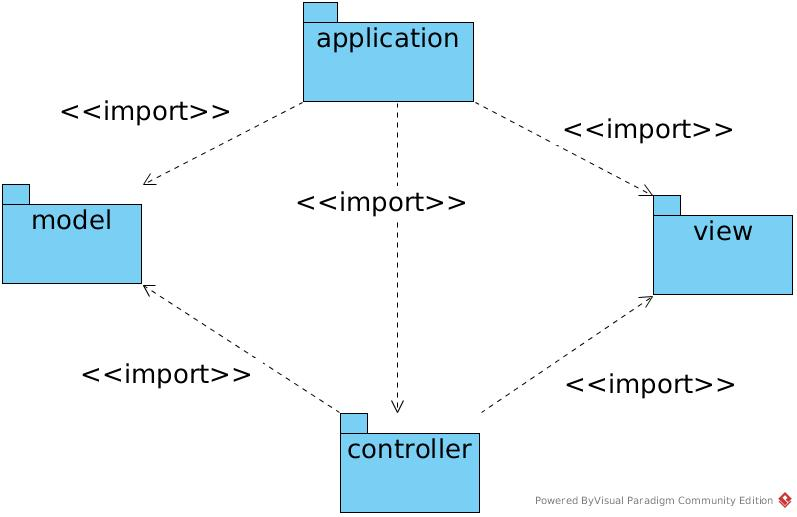
\includegraphics[scale = 0.4]{architecture}
\end{figure}

This project is separated in several packages. This is following the MVC (Model, View, Controller) pattern. 

Firstly, there's the view packages. All of the text printed is from this package. There's two classes in this package : DungeonView and MenuView. Their name speaks for themselves, the MenuView class displays all the text of the Menu and the other one, displays all the text for the game.

Then, the model package. This is the biggest one. It contains the classes and enumerations of all the elements used in the project. There's a lot of them so I'm not going to list them.

To complete our MVC, the controller package includes the model and the view packages to basically control them. It checks the state of the model to display the corresponding text from the view package.

Eventually, there's the application which only contains one class called Main. This class is the one executed to run the project. It's really simple and just calls the MenuController to start.

You can see it represented on figure \ref{architecture}.

\section{The scenario}

\begin{figure}[hb]
    \centering
    
    \caption{the menu}
    \label{menu}
    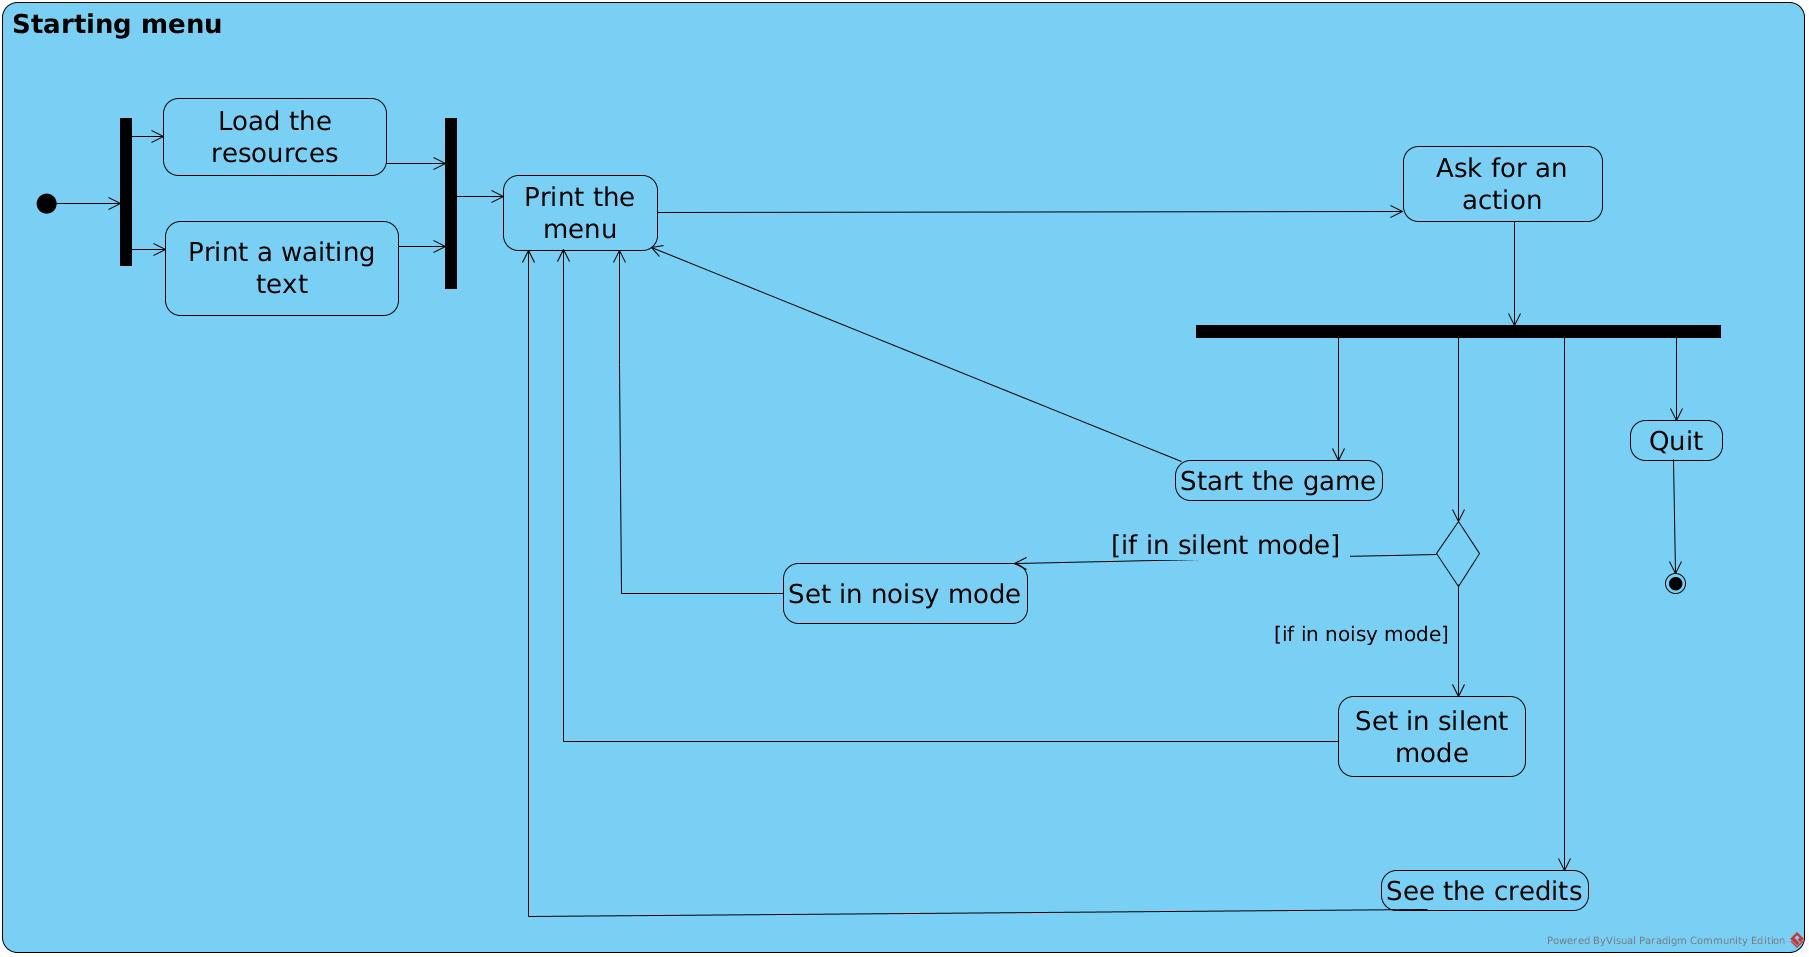
\includegraphics[scale = 0.198]{menu}
\end{figure}

When you run the application, you first have to wait until all the resources are loaded. Don't worry, you won't have to wait long everytime ! It detects whether the resources are already present on the computer. 

Once the resources are ready, the menu is displayed. It has four options and lets the user choose among them. After each choice, the menu is displayed again.

If the player has the game set in silent mode it would suggest to play it with sound and vice versa.

Once he is satisfied, he can start the game.

If needed, he can check the credits.

The user has also the posibility to quit through this menu. 

All of this is detailed in figure \ref{menu}.

\begin{figure}
    \centering
    
    \caption{the game}
    \label{game}
    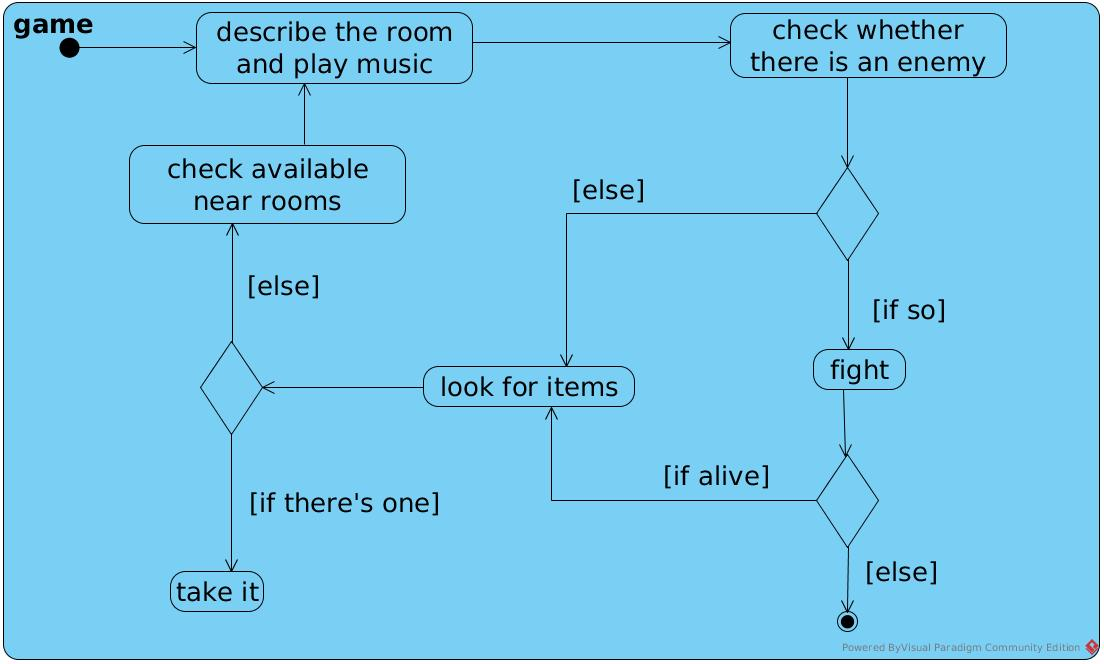
\includegraphics[scale = 0.32]{game}
\end{figure}

\vspace{\baselineskip}

Once the game is started, it continuously executes the following actions. It starts by describing the current room of the player and playing the music associated to the room. It then checks for the presence of an enemy in the room. If there's one, then there is a fight otherwise it just looks for items. If the player dies during the fight, the game is over. But if not, then we can go back to looking for items. It continuously look for one until there's none of them left. Once it's done, it checks the available rooms to go and restart it. You can see that in the figure \ref{game}.

\section{The loading of the resources}

\begin{figure}[t]
    \centering
    
    \caption{the loading of the resources}
    \label{resources}
    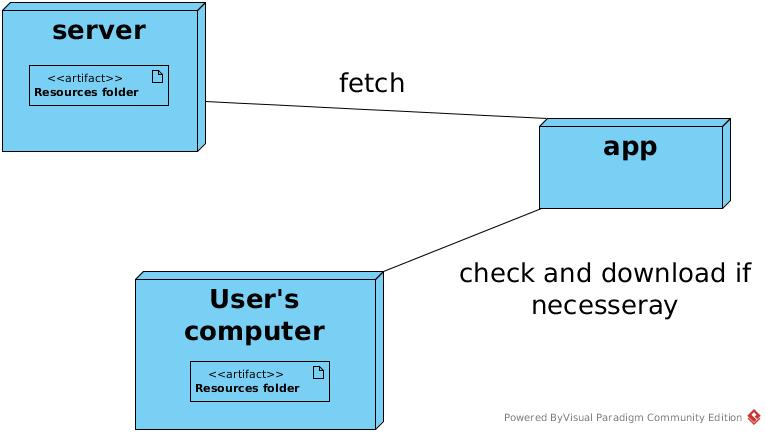
\includegraphics[scale = 0.46]{resources}
\end{figure}

All the resources for the game (which actually only contains the sounds) are stored on a server. The program fetches those data an recreate the corresponding folders present on the server to the user's computer. It also checks whether it already exists. 

This is shown in figure \ref{resources}.

\section{The menu}

\section{The main classes}

\section{The player's movement}

\section{The player's actions}

\section{The fight}

\part{My mistakes}

\part{Bonus}

\part{Conclusion}

\end{document}